This is the first sub section that user interacts with. When the user opens the mobile application for the first time details for SignUp is displayed. Then the user enters all the information required for SignUp including all the valid username and password to create a account. Then an account for the user is created.

\subsection{Input Validation}
This sub system just deals with the input validation. This subsystem is created to prevent form SQL injection. Input validation takes the input of the user and checks if the input is SQL query and discards if input is query or malicious input.

\begin{figure}[h!]
	\centering
 	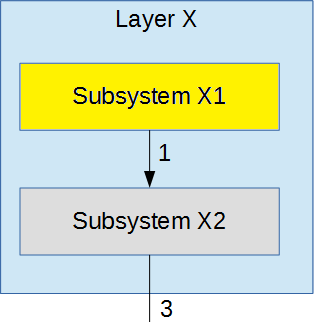
\includegraphics[width=0.60\textwidth]{images/subsystem}
 \caption{Example subsystem description diagram}
\end{figure}

\subsubsection{Assumptions}
Following assumptions are made for this SubSystem:
\begin{itemize}
    \item Inventory app is already installed on users cellphone.
    \item User provides some kind of input the form.
\end{itemize}

\subsubsection{Responsibilities}
Following are the responsibilities of this SubSystem:
\begin{itemize}
    \item This subsection must check if the input given by user is some type of SQL query.
\end{itemize}

\subsubsection{Subsystem Interfaces}
Each of the inputs and outputs for the subsystem are defined here. Create a table with an entry for each labelled interface that connects to this subsystem. For each entry, describe any incoming and outgoing data elements will pass through this interface.

\begin {table}[H]
\caption {Subsystem interfaces} 
\begin{center}
    \begin{tabular}{ | p{1cm} | p{6cm} | p{3cm} | p{3cm} |}
    \hline
    ID & Description & Inputs & Outputs \\ \hline
    \#xx & Description of the interface/bus & \pbox{3cm}{input 1 \\ input 2} & \pbox{3cm}{output 1}  \\ \hline
    \#xx & Description of the interface/bus & \pbox{3cm}{N/A} & \pbox{3cm}{output 1}  \\ \hline
    \end{tabular}
\end{center}
\end{table}

\subsection{Email/Password Validation}
This sub section just deals with the validation of username and password. This subsection makes sure that user enters the valid username and password while creating the account. For example email address must be followed by something.com and the password must contain at least 6 characters with upper case letter a number and a special character.

\begin{figure}[h!]
	\centering
 	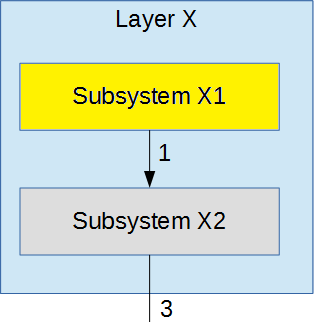
\includegraphics[width=0.60\textwidth]{images/subsystem}
 \caption{Example subsystem description diagram}
\end{figure}

\subsubsection{Assumptions}
Following are the assumption of SubSection Email/Password Validation:
\begin{itemize}
    \item Users cellphone is connected to the internet.
    \item User has a valid Email address.
    \item User provides the password that satisfies the basic password constrain. 
\end{itemize}
\subsubsection{Responsibilities}
Following responsibilities must be carried out by this SubSystem:
\begin{itemize}
    \item Email address must be validated. If Email address doesn't exist or is not valid, SubSystem must prevent form creating account.
    \item If the password doesn't meet minimum criteria, SubSystem must prevent user form creating account.
\end{itemize}

\subsubsection{Subsystem Interfaces}
Each of the inputs and outputs for the subsystem are defined here. Create a table with an entry for each labelled interface that connects to this subsystem. For each entry, describe any incoming and outgoing data elements will pass through this interface.

\begin {table}[H]
\caption {Subsystem interfaces} 
\begin{center}
    \begin{tabular}{ | p{1cm} | p{6cm} | p{3cm} | p{3cm} |}
    \hline
    ID & Description & Inputs & Outputs \\ \hline
    \#xx & Description of the interface/bus & \pbox{3cm}{input 1 \\ input 2} & \pbox{3cm}{output 1}  \\ \hline
    \#xx & Description of the interface/bus & \pbox{3cm}{N/A} & \pbox{3cm}{output 1}  \\ \hline
    \end{tabular}
\end{center}
\end{table}


\subsection{DB Controller}
This is the subsystem that deals with the database part of the Application. It is responsible for taking all the user input provided in the SignUp form and store it in the database accordingly.

\begin{figure}[h!]
	\centering
 	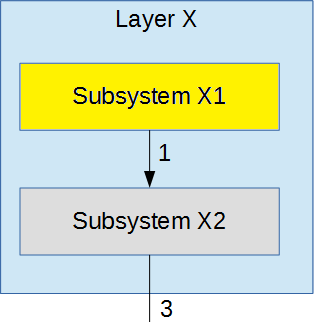
\includegraphics[width=0.60\textwidth]{images/subsystem}
 \caption{Example subsystem description diagram}
\end{figure}

\subsubsection{Assumptions}
Following assumptions are made about this 

\subsubsection{Responsibilities}
Each of the responsibilities/features/functions/services of the subsystem as identified in the architectural summary must be expanded to more detailed responsibilities. These responsibilities form the basis for the identification of the finer-grained responsibilities of the layer's internal subsystems. Clearly describe what each subsystem does.

\subsubsection{Subsystem Interfaces}
Each of the inputs and outputs for the subsystem are defined here. Create a table with an entry for each labelled interface that connects to this subsystem. For each entry, describe any incoming and outgoing data elements will pass through this interface.

\begin {table}[H]
\caption {Subsystem interfaces} 
\begin{center}
    \begin{tabular}{ | p{1cm} | p{6cm} | p{3cm} | p{3cm} |}
    \hline
    ID & Description & Inputs & Outputs \\ \hline
    \#xx & Description of the interface/bus & \pbox{3cm}{input 1 \\ input 2} & \pbox{3cm}{output 1}  \\ \hline
    \#xx & Description of the interface/bus & \pbox{3cm}{N/A} & \pbox{3cm}{output 1}  \\ \hline
    \end{tabular}
\end{center}
\end{table}

